\section{Tiradas de habilidad}

Las tiradas de habilidad se utilizan siempre que no haya otro sistema más específico aplicable. Interactúan principalmente con las habilidades y las características.

\subsection{Determinar la habilidad o característica}

Cuando exista una habilidad aplicable a la tirada, ésta tendrá prioridad sobre las características.

Consultar las listas de habilidades y características.

\subsection{Interpretar el resultado de una tirada}

Las tiradas de habilidad se realizan con 1D100, normalmente representado con 2D10 para decenas y unidades.

\vspace{-\parskip}

\begin{center}
\begin{tabular}{|c|c|}
    \hline
    Resultado                       & Interpretación            \\
    \hline
    1                               & Éxito crítico             \\
    $\leq$ $\sfrac{1}{5}$ habilidad & Éxito extremo             \\
    $\leq$ $\sfrac{1}{2}$ habilidad & Éxito difícil             \\
    $\leq$ habilidad                & Éxito normal              \\
    $>$ habilidad                   & Fracaso                   \\
    95-99                           & Pifia si habilidad $<$ 50 \\
    100                             & Pifia                     \\
    \hline
\end{tabular}
\end{center}

\subsection{Tiradas con dificultad}

Este tipo de tiradas requieren un nivel de éxito equivalente a su grado de dificultad. Son sensibles a éxitos críticos y pifias y en ocasiones también al nivel de éxito.

Las ventajas y desventajas alteran su dificultad.

\subsection{Tiradas enfrentadas}

Este tipo de tiradas enfrentan a dos personajes y comparan sus niveles de éxito. En caso de empate gana la habilidad o característica más alta. 

Las ventajas y desventajas aplican dados de bonificación o penalización a las decenas. Es decir, se lanza más de un dado y se utiliza solo el mejor o peor resultado.

\vspace{-1.5\parskip}

\begin{figure}[h]
    \centering
    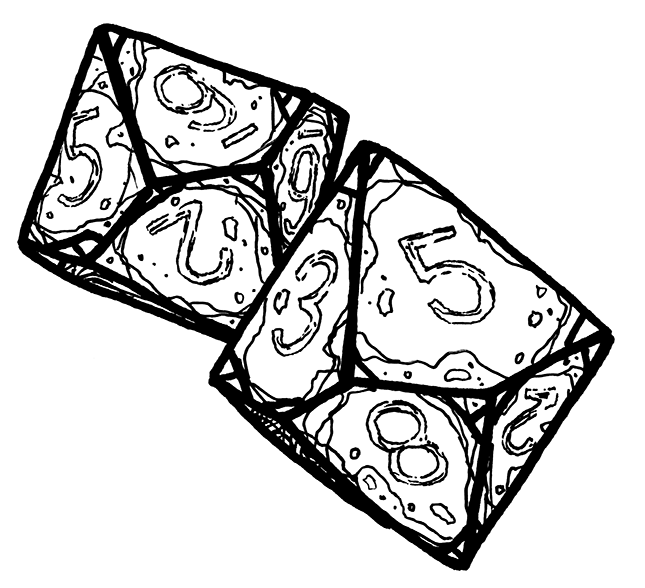
\includegraphics[width=0.19\textwidth]{images/2d10.png}
\end{figure}

\vspace{-2\parskip}

\subsection{Gastar suerte}

Es posible gastar tantos puntos de suerte como se desee para aumentar en esa cantidad el resultado de una tirada de habilidad. No es posible gastar suerte en una pifia.

\subsection{Forzar la tirada}

Cuando la acción de un personaje fracasa, es posible forzar una segunda tirada justificando un nuevo acercamiento. Volver a fracasar tendrá consecuencias graves.

No es posible gastar suerte en una tirada forzada.